% This is samplepaper.tex, a sample chapter demonstrating the
% LLNCS macro package for Springer Computer Science proceedings;
% Version 2.20 of 2017/10/04
%
\documentclass[runningheads]{llncs}
%
\usepackage{xcolor}
\usepackage{graphicx}
\usepackage{makecell}
\usepackage{textcomp}
%\usepackage{amsmath,amssymb,amsfonts}
\usepackage{algorithm,algorithmic}
\usepackage{wrapfig}
% Used for displaying a sample figure. If possible, figure files should
% be included in EPS format.
%
% If you use the hyperref package, please uncomment the following line
% to display URLs in blue roman font according to Springer's eBook style:
% \renewcommand\UrlFont{\color{blue}\rmfamily}

\renewcommand{\baselinestretch}{0.96}

\begin{document}
%
%\title{Automated Formal Synthesis of Optimal Sizing for Stand-alone Solar Photovoltaic Systems\thanks{Supported by Newton Fund (ref. 261881580) and FAPEAM (Amazonas State Foundation for Research Support, calls 009/2017 and PROTI Pesquisa 2018).}}
\title{Synthesis of Solar Photovoltaic Systems: Optimal Sizing Comparison\thanks{Supported by Newton Fund (ref. 261881580) and FAPEAM (Amazonas State Foundation for Research Support, calls 009/2017 and PROTI Pesquisa 2018).}}
%
%\titlerunning{Abbreviated paper title}
% If the paper title is too long for the running head, you can set
% an abbreviated paper title here
%
\author{Alessandro Trindade\inst{1} \and Lucas Cordeiro\inst{2}} %\orcidID{0000-0001-8262-2919}  \orcidID{0000-0002-6235-4272}
%
\authorrunning{A. Trindade and L. Cordeiro}
% First names are abbreviated in the running head.
% If there are more than two authors, 'et al.' is used.
%
\institute{Federal University of Amazonas, Brazil \email{alessandrotrindade@ufam.edu.br} \and
University of Manchester, UK \email{lucas.cordeiro@manchester.ac.uk}}
\maketitle              % typeset the header of the contribution

\begin{abstract}
The use of formal methods in electrical systems is a new subject, with significant research spanning only the last four years. However, the use of automated synthesis to obtain optimal sizing of solar photovoltaic (PV) systems remains unexplored in literature. Here our primary goal is to develop and evaluate a sound, automated synthesis approach to obtaining optimal sizing of stand-alone PV systems. We propose a variant of the counterexample guided inductive synthesis approach, with two phases linking the technical and the cost analysis. First, we synthesize a feasible candidate based on power reliability, which may not attain the lowest cost. Second, the candidate is then verified iteratively with a lower bound cost via symbolic model checking. If the verification step succeeds, the lower bound is adjusted; if it fails, a counterexample provides the optimal solution. Experimental results demonstrate that we can produce an optimal solution within an acceptable run-time. We also present a comparison with a specialized simulation tool over real PV systems to show the effectiveness of our approach.
%\keywords{Automated verification  \and Model Checking \and Solar photovoltaic systems.}
\end{abstract}

%%%%%%%%%%%%%%%%%%%%%%%%%%%%%%%%%%%%%%%%%%%%%%%%%%%%%%%%
\section{Introduction}
%%%%%%%%%%%%%%%%%%%%%%%%%%%%%%%%%%%%%%%%%%%%%%%%%%%%%%%%

Lack of access to clean and affordable energy is considered a core dimension of poverty~\cite{Hussein2012}. Progress has been made worldwide; in particular, in 2017, the number of people without electricity access fell below $1$ billion threshold for the first time~\cite{IEAweo2018}. In order to provide electricity for all, decentralized systems led by solar photovoltaic (PV) in off-grid and mini-grid systems will be the lowest-cost solution for three-quarters of the additional connections needed~\cite{Hussein2012}. 

In order to simulate or evaluate a PV system, there exist various specialized tools, e.g., RETScreen~\cite{Pradhan} and HOMER~\cite{Swarnkar}; and even general-purpose simulation tools, e.g., MATLAB/Simulink~\cite{Gow1999}. 
 However, these tools are based on simulation; they have the drawback of an incomplete coverage since verification of all possible combinations and potential failures of a system is unfeasible~\cite{ClarkeHV18}. 

Optimization of PV systems is not a recent topic; since the '90s, different techniques using different criteria to find ultimate combinations for design parameters, based on intuitive, numerical, and analytical methods, were proposed and developed~\cite{Alsadi2018}. In $2015$, an automated simulation-based verification technique was applied to verify the correctness of power system protection settings~\cite{Sengupta2015}. In $2017$, a researcher suggested the application of formal methods to verify and control the behavior of computational devices in a smart grid ~\cite{Abate2017}. In $2018$, a verification methodology was applied to PV panels and its distributed power point tracking~\cite{Driouich2018}. In $2019$, an automated verification methodology was proposed to validate stand-alone solar PV systems~\cite{TrindadeCordeiro19}. However, \textit{formal methods and its application to synthesize PV systems are still unexplored in literature}.

Here we developed a variant of the counterexample guided inductive synthesis (CEGIS)~\cite{DBLP:conf/asplos/Solar-LezamaTBSS06} technique for synthesizing optimal sizing of stand-alone PV systems using commercial equipment data. Given a correctness specification $\sigma$, our method uses that as a starting point and then iteratively produces a sequence of candidate solutions that satisfy $\sigma$, related to power reliability. In particular, on each iteration, we synthesize the sizing of stand-alone PV systems, but that may not achieve the lowest cost. The candidate solution is then verified via symbolic model checking with a lower bound that serves as the minimum cost of reference; if the verification step does not fail, the lower bound is adjusted. If it fails, then a counterexample is provided with an optimal sizing that meets both power reliability and system cost. 

Our work makes three significant contributions to advance the state-of-the-art in PV optimal sizing. First, the use of automated symbolic verification in PV systems was uncommon in recent prior studies~\cite{TrindadeCordeiro19}, and specifically, their use in synthesizing PV sizing is novel. Second, we evaluate our approach using different state-of-the-art symbolic verifiers to obtain the best performance in our verification back-end for synthesizing optimal PV systems and compare that to HOMER. Lastly, we discuss the main challenges of applying formal methods to PV systems and also reflect on lessons learned from this practical experience.

%-----------------------------------------------------------
\section{Preliminaries}
\label{sec:AutomatedVerification}
%-----------------------------------------------------------

Fig.~\ref{fig:optimization} illustrates how to obtain the optimal sizing of a stand-alone PV system using the traditional techniques (manual and simulation) and the proposed automated synthesis techniques. Note that the input information is the same for all the methods: weather data, price information, design requirements, as load curve and power demand, and design assumptions. For the automated synthesis, we also define the bound $k$ to restrict the design-space search. On the one hand, if $k$ is too small, then the approach might not return a solution due to the search-space depth. Here we start with a low bound $k$ and incrementally increase it to avoid time and memory constraints on our verification back-end. Therefore, the proper choice of $k$ is essential to this method.
%
\begin{figure}[h]
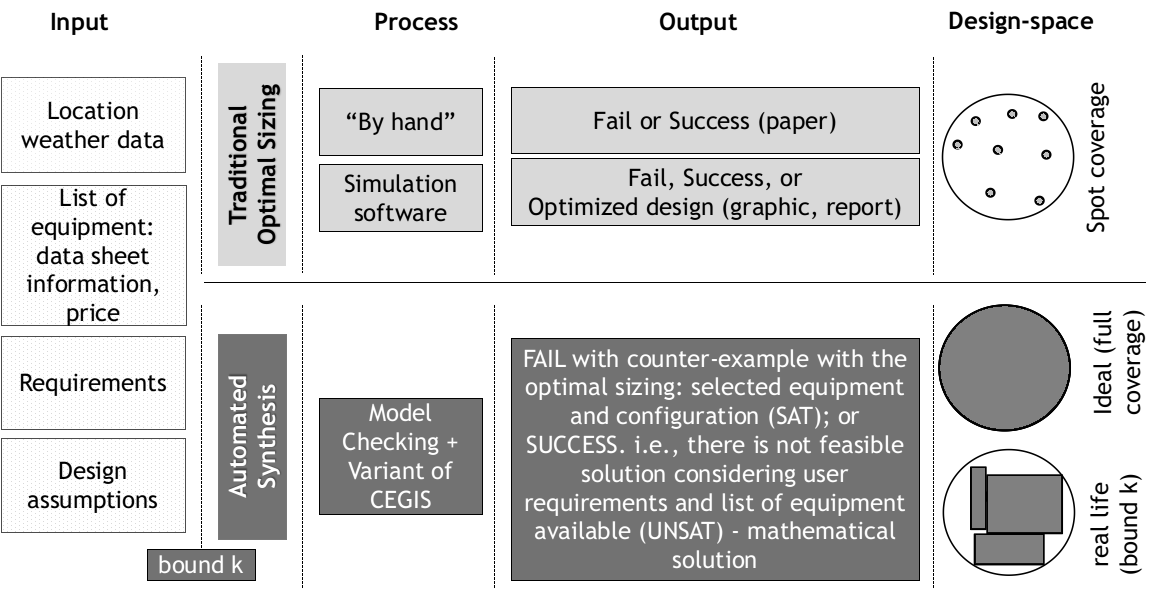
\includegraphics[width=0.8\textwidth]{optimalsizingprocess3}
\centering
\caption{Comparison of optimal sizing methods.}
\label{fig:optimization}
\end{figure}

Both techniques (traditional and automated synthesis)  produce as output either a SUCCESS or FAIL result, thereby considering a feasible technical solution with the lowest cost. On the one hand, when done by simulation, we get a report or graphical result; on the other hand, the automated synthesis technique, which is a mathematical reasoning of a model, presents a counterexample with the optimal solution stored in variables. Furthermore, the design-space coverage during the optimal sizing search is sound and complete when using synthesis.

%-----------------------------------------------------------
\subsection{Program Synthesis}
\label{sec:ProgramSynthesis}
%-----------------------------------------------------------

The basic idea of program synthesis is to automatically construct a program $P$ that satisfies a correctness specification $\sigma$. In particular, program synthesis is automatically performed by engines that use a correctness specification $\sigma$, as starting point, and then incrementally produce a sequence of candidate solutions that partially satisfy $\sigma$~\cite{Abateetal2017}. As a result, a given candidate program $p$ is iteratively refined to match $\sigma$ more closely. Figure~\ref{Counter-Example-Guided-Inductive-Synthesis} illustrates the underlying architecture. 
%
\begin{wrapfigure}{r}{0.5\textwidth}
\begin{center}
%\begin{figure}[h]
%	\centering
	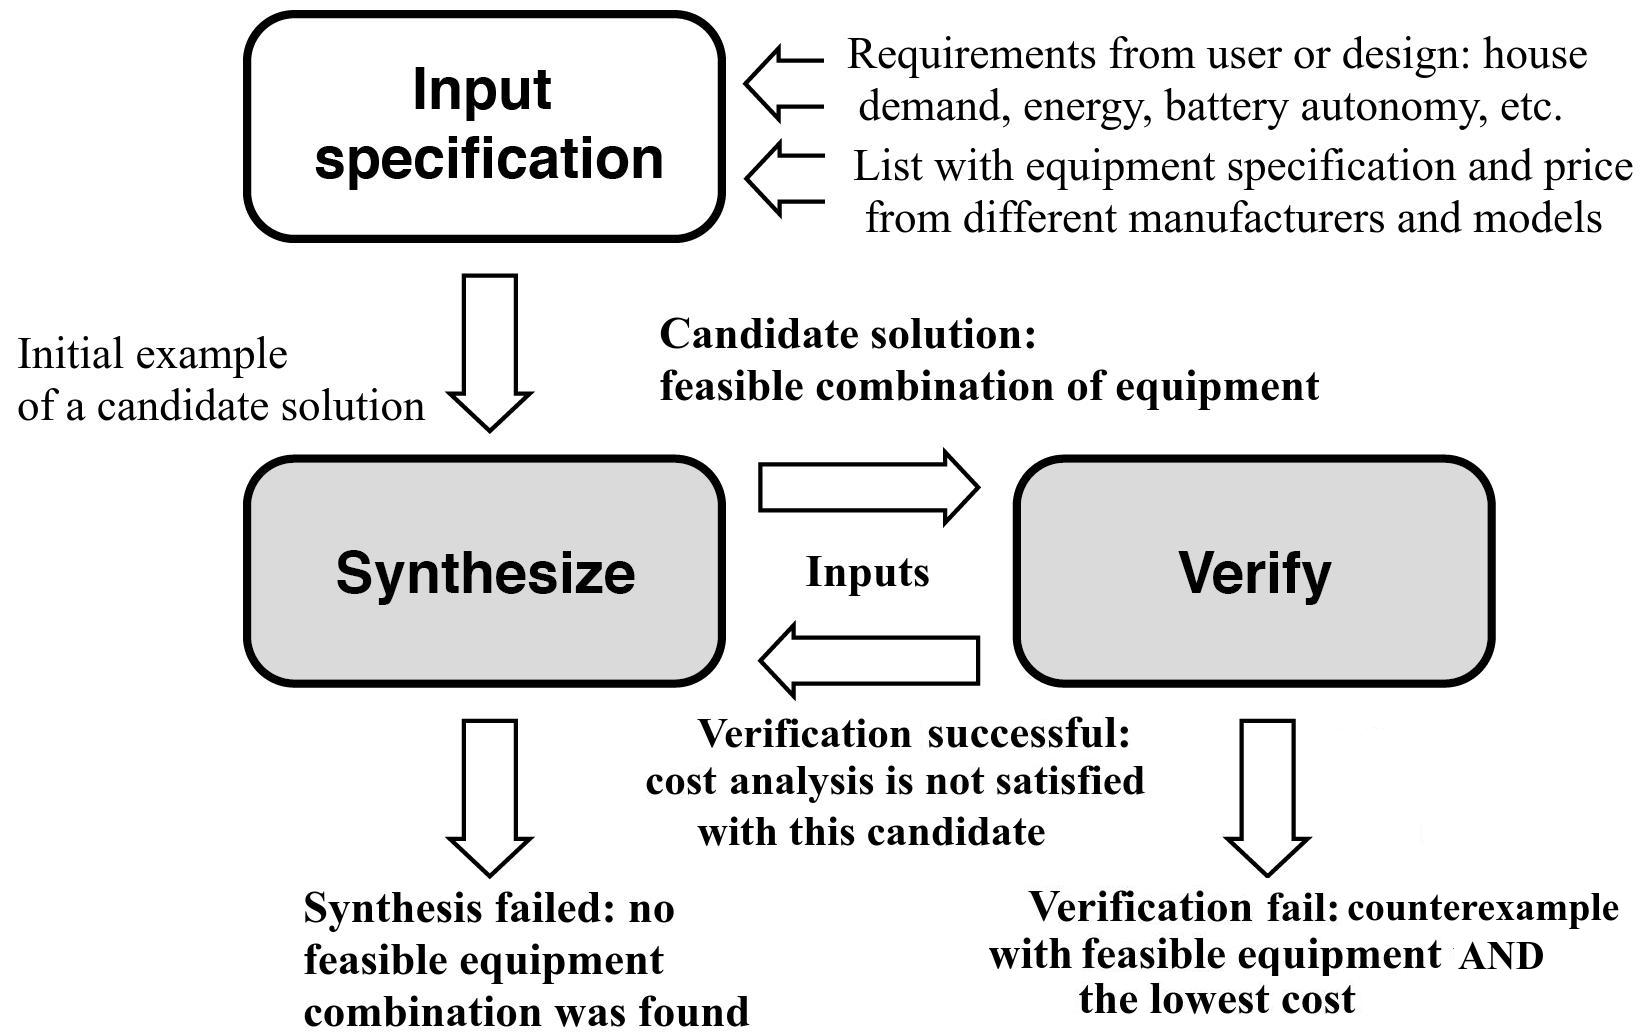
\includegraphics[width=0.5\columnwidth]{fig2_rev2.jpg}
\end{center}	
	\caption{CEGIS in PV system sizing.}
	\label{Counter-Example-Guided-Inductive-Synthesis}
%\end{figure}
\end{wrapfigure}

The correctness specification $\sigma$ provided to our synthesizer is of the form $\exists \vec{F}. \forall \vec{x}. \sigma(\vec{x}, \vec{F})$, where $\vec{F}$ ranges over functions, $\vec{x}$ ranges over ground terms, and $\sigma$ is a quantifier-free (QF) formula typically supported by SMT solvers. The ground terms are interpreted over some finite domain $\mathcal{D}$, where $\mathcal{D}$ can be encoded using the SMT's bit-vectors part. Our specification includes house demand, energy, and battery autonomy; we also provide equipment specifications and prices from different manufacturers and models.

In Figure~\ref{Counter-Example-Guided-Inductive-Synthesis}, regarding traditional CEGIS method, the phases {\sc Synthesize} and {\sc Verify} interact via a finite set of test vectors {\sc inputs}, which is incrementally updated. Given the correctness specification $\sigma$, the {\sc Synthesize} procedure tries to find an existential witness $\vec{F}$ satisfying the specification $\sigma(\vec{x}, \vec{F})$, for all $\vec{x}$ in {\sc inputs} (as opposed to all $\vec{x} \in \mathcal{D}$). If {\sc Synthesize} succeeds in finding a witness~$\vec{F}$, the latter is a candidate solution (i.e., feasible combination of equipment) to the full synthesis formula, which is passed to {\sc Verify} to check whether it is a proper solution ({\it i.e.}, $\vec{F}$ satisfies the specification $\sigma(\vec{x}, \vec{F})$ for all $\vec{x}\in\mathcal{D}$). If this is the case, then the algorithm terminates, i.e., we have found a feasible equipment with the lowest cost; otherwise, in the CEGIS traditional method, additional information is provided to the phase {\sc Synthesize}, in the form of a new counterexample that is added to the {\sc inputs} set and the loop iterates again.

One may notice that each iteration of the traditional CEGIS loop adds a new input to the finite set $INPUTS$, which is then used for synthesis. Given that the full set of inputs $\mathcal{D}$ is finite because we use bit-vector expressions, this means that the refinement loop can only iterate over a finite number of times. However, {\sc Synthesize} may conclude that no candidate solution obeying $\sigma$ for the finite set $INPUTS$ exists, and our synthesis engine can then conclude that no possible equipment combination was found.

In our CEGIS variant, there exist four differences related to the traditional one: 
(1) there exists no test vector and every candidate is generated during the run-time in the {\sc Synthesize} phase and sent to the {\sc Verify} phase; 
(2) if the {\sc Verify} phase is unsuccessful, then a new candidate is generated by {\sc Synthesize} and 
(3) the lower bound of the {\sc Verify} phase is incremented to search for the lowest cost; as a result,
(4) there exists no refinement from the {\sc Verify} phase back to the {\sc Synthesize} phase, i.e., 
a new counterexample is not added to the {\sc input} set since a failure during the {\sc Verify} phase will only discard a given candidate, which could be feasible in the next iteration with a new lower bound.%

%%%%%%%%%%%%%%%%%%%%%%%%%%%%%%%%%%%%%%%%%%%%%%%%%%%%%%%%
\subsection{Sizing Stand-alone Solar PV Systems}
\label{sec:sizing}
%%%%%%%%%%%%%%%%%%%%%%%%%%%%%%%%%%%%%%%%%%%%%%%%%%%%%%%%

A PV system is illustrated in Fig.\ref{fig:blockdiagram}. 
The PV generator, which can be a panel or an array, is a semiconductor device that can convert solar energy into DC electricity. 
For night hours or rainy days, we hold batteries where power can be stored and used. The use of batteries as a storage form implies the presence of a charge controller~\cite{Hansen}. The PV arrays produce DC, and therefore when the PV system contains an AC load, a DC/AC conversion is required. That converter is called inverter; the AC load dictates the behavior of the AC electrical load from the house that will be fed by the system.

\begin{wrapfigure}{r}{0.5\textwidth}
%\begin{figure}[h]
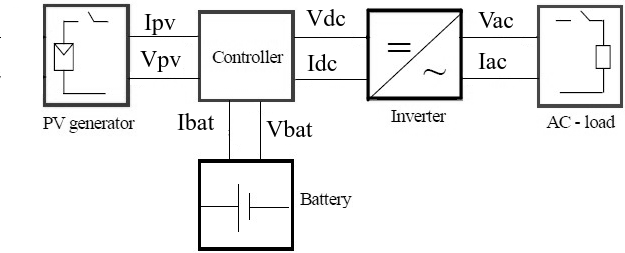
\includegraphics[width=0.5\textwidth]{blockdiagramPVS2_rev}
\centering
\caption{Block diagram for a typical stand-alone PV system~\cite{Hansen}.}
\label{fig:blockdiagram} 
\end{wrapfigure}

The sizing check will ensure that the system meets the standard project steps related to the critical period solar energy method~\cite{Pinho} and the MPPT (Maximum Power Point Tracking) charge controller, which is the most common one in practice. Firstly, we need to correct the energy consumption estimated to the load ($E_{consumption}$), which is carried out by Eq.~\ref{eq:Ecorrected}, where the efficiency of batteries ($\eta_{b}$), controller ($\eta_{c}$), and inverter ($\eta_{i}$) are considered~\cite{Pinho} as follows

\begin{equation}
\label{eq:Ecorrected}
E_{corrected} = \frac {E_{consumption}}{\eta_{b} \eta_{c} \eta_{i} }.
\end{equation}

We also need to estimate the energy that can be produced for each panel, called $E_{p}$, in Wh, defined as

\begin{equation}
\label{eq:Ep}
E_{p} = Solar\_Irradiance \times Panel\_Area \times \eta_{p} \times 1000,
\end{equation}

\noindent where the solar irradiance is expressed in terms of $kWh/m^{2}$ and depends on the site where the PV system will be deployed; 
the PV panel area is given in $m^{2}$ and corresponds to the size of one PV panel, and $\eta_{p}$ represents the PV panel efficiency.
The minimum number of solar panels ($N_{TPmin}$) is computed as

\begin{equation}
\label{eq:NTPmin}
N_{TPmin} = \frac{E_{corrected}}{E_{p}}.
\end{equation}

Notably, the total number of panels in series ($N_{PSmin}$) and parallel ($N_{PPmin}$) are respectively given by

\begin{equation}
\label{eq:NPSmin}
\frac{V_{mppt,min}}{V_{maxPower,TempMax}} \leq N_{PSmin} \leq \frac{V_{mppt,max}}{V_{maxPower,TempMin}},
\end{equation}

\begin{equation}
\label{eq:NPPmin}
N_{PPmin} = \frac{P_{total}}{Number\,Panels\,Series \times P_{max,ref}},
\end{equation}

\noindent where $V_{mppt, max}$ is the maximum operation voltage and $V_{mppt,min}$ is the minimum operating voltage of the charge controller. $V_{maxPower, TempMax}$, as well as $V_{maxPower, TempMin}$, are the maximum power voltage from the PV module considering the maximum and minimum operational temperature, respectively. $P_{total}$ is the total power demanded from the PV system and $P_{max, ref}$ is the power supplied from one PV panel in $Watts$. Regarding batteries, we must first define the total capacity of the battery bank, which can be described as

\begin{equation}
\label{eq:Cbank}
C_{bank} = \frac{E_{corrected} \times autonomy}{V_{system} \times DOD},
\end{equation}

\noindent where the variable $autonomy$ is a design definition; 
$ V_{system} $ is the DC voltage of the bus, and $ DOD $ is the battery depth of discharge (considered of maximum of 25\% here).
Secondly, the total (minimum) number of batteries $N_{B}total$ is computed as a product of the minimum number of batteries in series $N_{BS}min$ with the minimum number of batteries in parallel $ N_{BP}min $ and, therefore, as function of battery bank capacity $ C_{bank} $ and the capacity of the chosen battery $ Battery \, Capacity $ as

\begin{equation}
\label{eq:Nbtotal}
N_{B}total = N_{BS}min \times N_{BP}min = \frac{V_{system}}{V_{bat}} \times \frac{C_{bank}}{Battery \, Capacity}.
\end{equation}

Regarding the charge controller, it must initially meet the voltage requirement of the PV system $V_{system}$, as described by Eq.~\ref{eq:vcvsystem} to the charge controller voltage $V_{c}$: 

\begin{equation}
\label{eq:vcvsystem}
V_{c} = V_{system}.
\end{equation}

The short circuit reference current $ I_{sc,ref} $ from the manufacturer's solar panel must be corrected to the cell temperature because the field temperature $ T $ is higher than the nominal or laboratory temperature, and PV system is temperature dependent. This corrected current is called $I_{sc,amb}$, it uses $G_{ref} = 1000$ and the ratio of current change over temperature $\mu_{I}$:

\begin{equation}
\label{eq:iscamb}
I_{sc,amb} = \frac{Solar \, Irradiance}{G_{ref}} \left[I_{sc,ref} + \mu_{I} \times (T-25) \right]. 
\end{equation}

The controller must meet the maximum current from the PV array. Therefore the controller current $I_{c}$ must be less than the calculated $I_{c,min}$ and given as
%
\begin{equation}
\label{eq:icmin}
I_{c,min} = I_{sc,amb} \times N_{PP},
\end{equation}

\begin{equation}
\label{eq:icicmin}
I_{c} \geq I_{c,min}.
\end{equation}

The inverter sizing check is performed by means of three equations. Eq.~\ref{eq:vindc} ensures that the input voltage of the controller $V_{in}DC$ meets the system voltage. Eq.~\ref{eq:voutac} ensures that the output voltage of the controller $V_{out}AC$ meets the AC voltage of the load $V_{AC}$. Finally, Eq.~\ref{eq:invcheck} ensures that the controller can support the total demand of the load ($Demand$) and the surge power ($P_{surge}$), where $V_{in}DC$ is the nominal input voltage and $V_{out}AC$ is the nominal output voltage of the inverter; $P_{AC,ref}$ is the nominal power and $MAX_{AC,ref}$ is the peak power that the inverter can support.

\begin{equation}
\label{eq:vindc} 
V_{in}DC = V_{system}.
\end{equation}

\begin{equation}
\label{eq:voutac} 
V_{out}AC = V_{AC}.
\end{equation}

\begin{equation}
\label{eq:invcheck} 
\left[ (Demand \leq P_{AC,ref}) \, and \, (P_{surge} \leq MAX_{AC,ref}) \right].
\end{equation}

All the equations above model the continuous-time behavior of the PV system; they produce real numbers, but when choosing batteries and panels quantities, those real numbers must be converted into integer numbers (closest ones, considering the minimum or maximum according to each equation). The underlying verification and simulation tools need to handle non-linear real arithmetic to produce the correct result.

%------------------------------------------------------
\section{Synthesizing Optimal Sizing of Stand-alone Solar Photovoltaic Systems}
%------------------------------------------------------

The optimal sizing of PV systems is made by the best compromise between two objectives: power reliability and system cost~\cite{Alsadi2018}. 
Regarding power reliability, this work will rely on the critical period solar energy method~\cite{Pinho}, as described in Section~\ref{sec:sizing}. 
Considering the system cost analysis, based on the fact that the deployment location is not specified, our study uses an adapted Life Cycle Cost (LCC) analysis, where only the acquisition cost is considered in the model, i.e., without the operational and maintenance costs~\cite{Alsadi2018}.

Algorithm~\ref{alg:verification-algorithm} describes our pseudo-code to synthesize stand-alone PV systems using symbolic model checking. 
%
 \begin{algorithm}
 \caption{Synthesis algorithm}
 \begin{algorithmic}[1]
 \begin{scriptsize}
 \renewcommand{\algorithmicrequire}{\textbf{Input:}}
 \renewcommand{\algorithmicensure}{\textbf{Output:}}
  \REQUIRE weather data (temperature, solar irradiance), list of equipment (datasheet and price information), design requirements (load curve, peak demand, output voltage, battery autonomy), design assumptions (battery state of charge, criteria and objectives for technical and cost analysis).
 \ENSURE FAIL with counter-example showing the optimal sizing; SUCCESS, saying that the project has no feasible solution considering the requirements and the list of equipment available.
 \STATE Initialize variables \\
 \STATE Declare list of PV panels, controllers, batteries, and inverters data and cost \\
 \STATE Declare the maximum possible cost $MaxCost$ \\
 \STATE Declare power demand, power peak, energy consumption \\
 \STATE Declare battery autonomy, depth of discharge, AC voltage \\
 \FOR {$HintCost=0$ to $MaxCost$}
 	\STATE Declare non-deterministic variable to select PV Panel from list \\
 	\STATE Declare non-deterministic variable to select Controller from list \\
 	\STATE Declare non-deterministic variable to select Battery from list \\
 	\STATE Declare non-deterministic variable to select Inverter from list \\ 	
 	\STATE Calculate $E_{corrected}, \, E_{p} $ \\
	\STATE Calculate $N_{TPmin}, \, N_{PSmin}, N_{PPmin} $ \\
 	\STATE Calculate $C_{bank}$ \\
	\STATE Calculate $N_{BS}min, \, N_{BP}min, \, N_{B}total$ \\
	\STATE Requirement enforced by \textbf{assume}$(V_{c})$ \\
 	\STATE Calculate $I_{sc,amb}$ \\
 	\STATE Calculate $I_{c,min}$ \\
 	\STATE Requirement enforced by \textbf{assume}$(I_{c} \wedge V_{in}DC \wedge V_{out}AC)$ \\
	\STATE Requirement enforced by \textbf{assume}$(Demand \wedge P_{surge})$ \\
	\STATE non-deterministic variables hold feasible equipment and cost \\
	\STATE $F_{obj} \leftarrow N_{TP}*Panel_{Cost} \, + \, N_{TB}*Battery_{Cost} \, + Controller_{Cost} \, + \, Inverter_{Cost}$ \\
	\STATE Violation check with \textbf{assert}$(F_{obj} > HintCost)$ \\
 \ENDFOR
 \RETURN $(\,)$ 
 \end{scriptsize}
 \end{algorithmic} 
 \label{alg:verification-algorithm}
 \end{algorithm}
%
Our synthesis algorithm will synthesize constant values; it starts with the input of manufacturers' data and prices of PV panels, batteries, charge controllers, and inverters (Line 2). We define user requirements, i.e., house requirements and design definitions, from Lines 4 and 5. 

The \textit{for}-loop started at Line 6 controls the lowest cost to the PV solution. In particular, it starts with cost $0$ and stops only when the algorithm finds a feasible solution in which the cost breaks the $assertion$ stated in Line 22; if that happens, then our algorithm has found an optimal solution, thereby stating that the {\sc Verify} phase reached a satisfiable condition (\textit{SAT}). The $MaxCost$ value at Line 6 is just a very high value put as a limit to the \textit{for}-loop, which will never be reached because the optimal solution will be found first.

Our synthesis algorithm uses non-deterministic variables to choose one specific constant from a given list of PV panels, controllers, batteries, and inverters (Lines 7 to 10). That procedure ensures that our synthesis engine checks all combinations of items from each equipment, and combine them to assemble a feasible (candidate) PV solution, which meets the user requirements.
%
Next, we use Eq.~\ref{eq:Ecorrected}, Eq.~\ref{eq:Ep}, Eq.~\ref{eq:NTPmin}, Eq.~\ref{eq:NPSmin}, Eq.~\ref{eq:NPPmin}, Eq.~\ref{eq:Cbank}, Eq.~\ref{eq:Nbtotal}, Eq.~\ref{eq:iscamb}, and Eq.~\ref{eq:icmin} to calculate the sizing variables (Lines 11 to 17). The directive \textit{assume} (Lines 15, 18 and 19) ensures the compatibility of the chosen items from the list of equipment: the {\sc Verify} phase uses only the item (among all the possible ones) that satisfies the statements of Lines 15, 18, and 19. Our algorithm reaches Line 20 with one feasible solution; the cost of that solution is calculated in $F_{obj}$ (Line 21). 

If our algorithm does not find a feasible solution among the item of equipment that was provided to our {\sc Synthesize} phase, then the result is an unsatisfiable (\textit{UNSAT}), i.e., the program finishes and does not find a solution. It indicates that it was not possible to combine the items of each equipment and create a feasible solution. The main challenge for the {\sc Synthesize} phase is to find a feasible candidate solution regarding the constraints and user requirements. Related to our {\sc Verify} phase, the challenge is to find the lowest acquisition cost from a list of equipment and components that are provided from the {\sc Synthesize} phase. 
The process described here is entirely automated; a validation is performed by our {\sc Verify} phase to ensure that the approach is sound.

%---------------------------------------------------------------------------
\section{Results and Discussion}
%---------------------------------------------------------------------------
%---------------------------------------------------------------------------
\subsection{Description of the Case Studies}
%---------------------------------------------------------------------------

The proposed synthesis approach was evaluated in seven stand-alone PV system case studies. Here we report each case study as a tuple \textit{\{power peak (W); power surge (W); energy consumption (Wh/day); battery autonomy (hours)\}} as follows:
\textbf{case study 1:} \{342; 342; 3,900; 48\}; \textbf{case study 2:} \{814; 980; 4,880; 48\}; \textbf{case study 3:} \{815; 980; 4,880; 12\}; \textbf{case study 4:} \{253; 722; 3,600; 48\}; \textbf{case study 5:} \{263; 732; 2,500; 48\}; \textbf{case study 6:} \{322; 896; 4,300; 48\}; \textbf{case study 7:} \{1,586; 2,900; 14,000; 48\}.
These case studies were defined based on the usual electrical load found in riverside communities in the State of Amazonas, Brazil~\cite{TrindadeCordeiro19,Agrener2013}, except for case 7, which was idealized as a small-town solution to support a few lamps and a 12k BTUs air-conditioner. For all cases, an estimated load curve (kWh) was defined based on the electronics consumers in each house. Our synthesis algorithm was fed with data and costs of forty equipment items from ten different manufacturers of PV systems. 

Three start-of-the-art verification tools, CBMC\footnote{Command-line: \$ cbmc -\phantom{}-unwind 100 filename.c -\phantom{}-trace} version 5.11 with MiniSat 2.2.1~\cite{Kroening}, ESBMC\footnote{Command-line: \$ esbmc filename.c -\phantom{}-no-bounds-check -\phantom{}-no-pointer-check -\phantom{}-unwind 100 -\phantom{}-boolector} version 6.0.0 with the  Boolector 3.0.1 solver~\cite{Brummayer}, and CPAchecker\footnote{Command-line: \$ scripts/cpa.sh -heap 64000m -config config/bmc-incremental.properties -spec config/specification/sv-comp-reachability.spc filename.c} version 1.8 with MathSAT 5.5.3~\cite{mathsat5}, were used as verification engines to compare the proposed approach effectiveness and efficiency. 

%---------------------------------------------------------------------------
\subsection{Simulation Tool and Assumptions}
%---------------------------------------------------------------------------

Concerning the off-the-shelf simulation tools, only HOMER Pro performs off-grid system with battery backup analysis and includes economical analysis. Here we used HOMER Pro version $3.13.1$ as a state-of-the-art simulation tool for comparison purposes. In particular, HOMER Pro has the following characteristics:

\begin{itemize}
\item It is available only for MS Windows; its annual standard subscription costs US\$ $504.00$~\cite{HOMER}; 
\item It does not have LCC cost in its reports, only Net Present Cost (NPC); however, we can obtain LCC from NPC; 
\item The optimization analysis of HOMER defines a load curve and temperature according to data collected from online databases. However, to allow a correct comparison, the curve load and the temperature were defined the same as our synthesis approach; 
\item It does not have a charge controller. During the tests, we have chosen the ``load-following'' option, which produces enough power to meet the demand~\cite{HOMER} and (usually) presents a non-overestimated solution; 
\item It was assumed the value of 95\% availability of the PV system. By definition, ``availability'' is the percentage of time at which a power system can feed the load requirements~\cite{Khatib2014}. For ordinary house electrical load, 95\% is considered acceptable;
\item It was assumed a string of two batteries to match the voltage of the system of $24$ V DC, which was used for our automated synthesis tool; 
\item It was included a generic flat-plate PV of $1$ kW and generic lead-acid batteries of $1$ kW as well (and with capacity of $83.4$ Ah according to HOMER Pro modeling). During run-time, HOMER decides the size in kW of each module based on feasibility and lower cost.
\end{itemize}

%---------------------------------------------------------------------------
\subsection{Objectives and Setup}
%---------------------------------------------------------------------------

Our evaluation aims to answer three experimental goals: 
\begin{enumerate}
\item[EG1] \textbf{(soundness)} Does our automated synthesis approach provide correct results?, 
\item[EG2] \textbf{(performance)} How do the software verifiers compare to each other for synthesizing PV systems?, and 
\item[EG3] \textbf{(state-of-the-art)} how does our formal synthesis tool compare to a specialized simulation tool?
\end{enumerate}


All experiments regarding the verification tools were conducted on an otherwise idle Intel Xeon CPU E5-4617 ($8$-cores) with $2.90$ GHz and $64$ GB of RAM, running Ubuntu $16.04$ LTS $64$-bits. For HOMER Pro, we have used an Intel Core i5-$4210$ ($4$-cores) with $1.7$ GHz and $4$ GB of RAM running Windows 10. The hardware platform was not the same because of the availability of the machines; this has an impact on performance, which is less favorable to HOMER Pro.. We perform the experiments with a predefined time out of $240$ minutes.

%---------------------------------------------------------------------------
\subsection{Results}
%---------------------------------------------------------------------------
%A Table with the details of the results is present on-line\footnote{\url{https://drive.google.com/file/d/1I1Cg4FNz9grMqXHUmOKnd-\_PFmLpmk6m/view?usp=sharing}}. 

Concerning the verifiers' comparison, CPAchecker was able to synthesize the optimal sizing in six out of seven case studies (cases $1$ to $6$): CPAchecker produced the results within the time limit, which varied from $2.24$ to $3.92$ hours. Only case study $7$ led to a \textit{time out} result in CPAchecker. The violation (SAT result) indicated in the on-line table\footnote{\url{https://drive.google.com/file/d/1I1Cg4FNz9grMqXHUmOKnd-\_PFmLpmk6m/view?usp=sharing}} is the $assert$ of Line $22$ at Algorithm~\ref{alg:verification-algorithm}. CBMC and ESBMC are unable to produce any conclusive results since \textit{time-outs} or \textit{memory-outs} occurred; these results partially answer the \textit{EG1} and \textit{EG2}, because there exist optimal solutions for these case studies and CPAchecker presented the best results among the verifiers. 

In general, the size of the PV panels and battery bank were larger in HOMER Pro than with our synthesis approach. To compare the results obtained from the optimization, the authors have four PV systems deployed and monitored since June $2018$ in a riverside community in the Amazonas State, Brazil, with similar demands presented by case studies $1$, $4$, $5$, and $6$, with a configuration of $3$ $\times$ $325$ W ($3$S) panels and $4$ $\times$ $220$ Ah ($2$S-$2$P $= 440$ Ah) lead-acid batteries. These deployed systems are closer to the result presented by the proposed formal synthesis approach than HOMER Pro, thereby showing that the solution is sound, which answers \textit{EG1}.

For the inverters, HOMER Pro suggests a value in kW very close to the peak of every case study, and it is just a reference value and not a commercial value of the employed inverter. The proposed synthesis tool, however, presents inverters that are commercial and can be found off-the-shelf. Therefore, this feature is a PRO to the formal synthesis method. Concerning the charge controllers, HOMER Pro does not include it as an explicit equipment in its mathematical model, only the synthesis tool presents a commercial controller and includes it during the cost analysis. Therefore, the formal synthesis method presents more reliable results than HOMER Pro. Case study $7$ was not solved by the synthesis tool within the time limit established during the experimental phase. HOME Pro was unable to simulate case study $3$ since it does not have the feature of adjusting the battery autonomy, i.e., the tool always tries to feed with electricity the given load during $365$ days/year. This lack of recourse is a limitation since it is usual to establish autonomy as a design requirement.

In terms of performance, HOMER Pro was able to evaluate six case studies (cases $1$, $2$, $4$, $5$, $6$, and $7$) within a time shorter than $30$ seconds, which was faster than the proposed synthesis approach (cf.~\textit{EG3}) but not sound as our method.  
Comparing the results between the formal synthesis with CPAchecker and HOMER Pro, we have observed that the cost was very close in cases $1$, $4$, $5$ and $6$, with difference varying from $0.23$\% to $17.4$\%. However, HOMER Pro does not use costs related to charge controllers, which were introduced into our synthesis model. This charge controller cost makes the synthesis approach more precise and real. We observed that there exists a divergence in case study $2$, where the costs presented by HOMER Pro were $54$\% higher than our synthesis tool. However, this case study does not have a deployed PV system in order to validate which result is correct.

%---------------------------------------------------------------------------
\subsection{Threats to validity} 
%---------------------------------------------------------------------------

We have reported a favorable assessment of the proposed method. Nevertheless, we have also identified four threats to the validity of our results that can be further assessed and constitute future work: (1) improvement of the power reliability analysis: to include loss of load probability or loss of power supply probability, which can make the analysis more accurate; (2) improvement of the system cost analysis by including operational and maintenance costs to the adopted LCC analysis; (3) to increase the equipment and manufacturers database: this will increase the complexity of the optimization, but the result will also allow improved sizing; and (4) to compare the results of our approach with an off-the-shelf PV sizing/optimization software: this comparison will validate the results obtained, and it allows a simulation-verification comparison.

%------------------------------------
\section{Conclusion} 
%------------------------------------

Our novelty relies on a practical approach to pursuit the optimal solution of PV systems using formal methods. The use of formal synthesis has no precedent in literature, and we show that the results of our approach, using seven case studies, are promising.
Our synthesis tool can present a solution, which is far detailed and closer to the commercial reality than the solution presented by HOMER Pro, an state-of-the art simulation tool. The use of data from real deployed systems in Amazonas State, Brazil, were important in order to reach that conclusion. The battery autonomy feature of our synthesis approach is an advantage as well. In addition, our automated synthesis method can provide all the details of every component of a PV system solution, with complete electrical details from datasheet of manufacturers, including the model of the component, nominal current, and voltage. These details are important for the owner of the system and aids the process of equipment purchase.
%
% ---- Bibliography ----
% BibTeX users should specify bibliography style 'splncs04'.
% References will then be sorted and formatted in the correct style.
%
\bibliographystyle{splncs04}
\bibliography{trindadeThesis}
%
\end{document}
%\subsection{Design and Simulation of Solar PV systems}
%The design and validation of a PV system can be done by hand or with the aid of a software tool. In order to address different aspects of the PV system design, there are various software tools available in the literature~\cite{Rajanna,Rawat}.
%public domain and commercial software available for the PV market. 
%According to \cite{Brooks}, t
%%%%%%%%%%
%
%The capabilities of tools available in the literature range from simple solar resource and %energy production estimation, %to site survey and system design tools,
%to complex financial analysis and project optimization. At this study, the commercial simulation tool HOMER PRO was selected to be used at the case studies in order to be compared with the automated verification tools.
